\documentclass[tikz,border=2pt]{standalone}
\usepackage{amsmath,amssymb}
\usepackage{pgfplots}
\pgfplotsset{compat=1.18}

\begin{document}
% Densities of the three order statistics of n = 3 iid Unif(0,1) observations:
% minimum 3(1-x)^2, median 6x(1-x), maximum 3x^2.
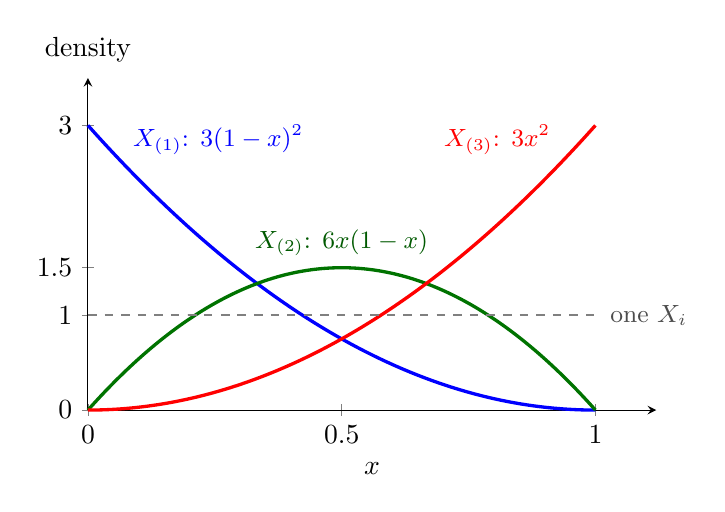
\begin{tikzpicture}
	\begin{axis}[
		axis lines=left, xmin=0, xmax=1.12, ymin=0, ymax=3.5,
		xtick={0,0.5,1}, ytick={0,1,1.5,3},
		xlabel={$x$}, ylabel={density}, ylabel style={rotate=-90, anchor=south, at={(axis description cs:0,1.02)}},
		samples=100, smooth, width=8.8cm, height=5.8cm, clip=false
		]
		\addplot[blue, very thick, domain=0:1] {3*(1-x)^2};
		\addplot[green!45!black, very thick, domain=0:1] {6*x*(1-x)};
		\addplot[red, very thick, domain=0:1] {3*x^2};
		\addplot[gray, dashed, thick, domain=0:1] {1};
		\node[blue, anchor=west, font=\small] at (axis cs:0.07,2.85) {$X_{(1)}$: $3(1-x)^2$};
		\node[green!35!black, anchor=south, font=\small] at (axis cs:0.5,1.52) {$X_{(2)}$: $6x(1-x)$};
		\node[red, anchor=east, font=\small] at (axis cs:0.93,2.85) {$X_{(3)}$: $3x^2$};
		\node[gray!60!black, anchor=west, font=\small] at (axis cs:1.01,1) {one $X_i$};
	\end{axis}
	
\end{tikzpicture}
\end{document}
